\review{The authors have addressed many of my previous comments. However, there are still several major issues that need further clarification.}

\vspace{1eM}
\underline{\textit{Reply:}} We thank the reviewer for providing further useful comments which help us to greatly improve the manuscript.

\begin{enumerate}
	
\cmnt{1} \review{The revised paper did not address my previous comment about how to select the sub-channel ordering. I understand that finding the best sub-channel ordering requires exhaustive search which has extremely high complexity. But it is important to provide a guidance on what would be a good choice of sub-channel ordering. For example, can we achieve a good performance by using a low complexity ordering algorithm such as a greedy sub-channel ordering algorithm?}

\resp We apologize for not clarifying the sub-channel ordering in detail in our previous manuscript. For simplicity we use random sub-channel ordering in our paper. That is, after finding the precoders for a current sub-channel, we can choose any previously unselected sub-channels as the next candidate sub-channel for which the precoders are identified using the updated backlogged packets. As suggested by the reviewer, the greedy sub-channel ordering can also be considered while selecting the order. The greedy ordering can be based on sorting the best channel gain from each sub-channel, which is obtained by finding the highest channel norm seen between any user and the corresponding serving \ac{BS}. However, note that the interference among the neighboring users are not included in this procedure, since the precoders that are required to evaluate the interference are designed after the sub-channel selection step only.
\begin{figure*}[h!]
	\centering
	\subfloat[][Number of backlogged packets for each user in bits \eqn{Q_k = [11,8,14,6,6,2,10,10,5,6,9,5]}]{
		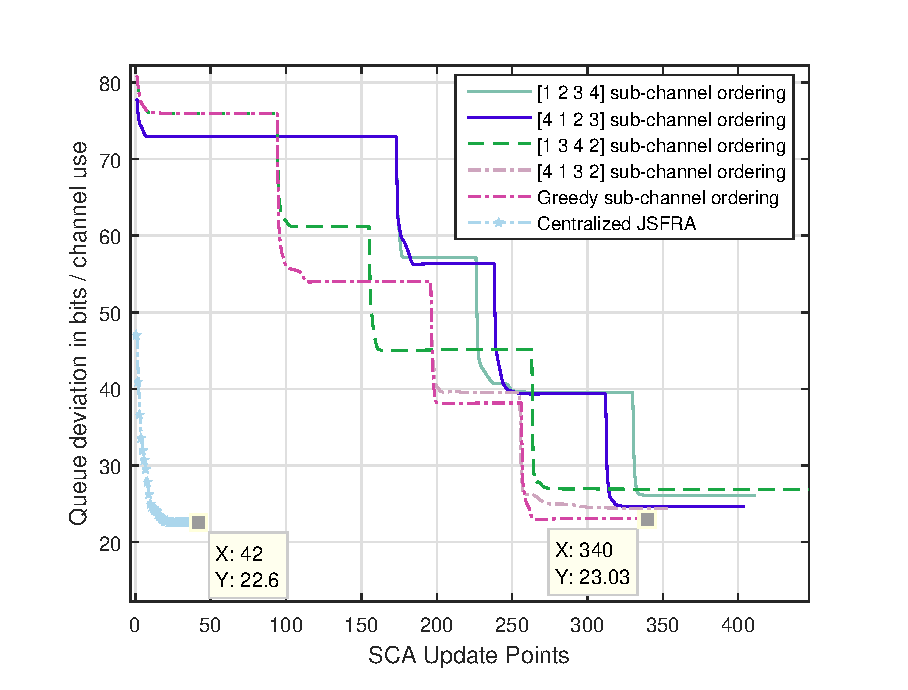
\includegraphics[width=0.8\textwidth]{reviewer_2_Q1B.eps}
		\label{fig-review-1a}
	}
	\hfill
	\subfloat[][Number of backlogged packets for each user in bits \eqn{Q_k = [8,9,12,8,12,5,4,10,8,5,7,9]}]{
		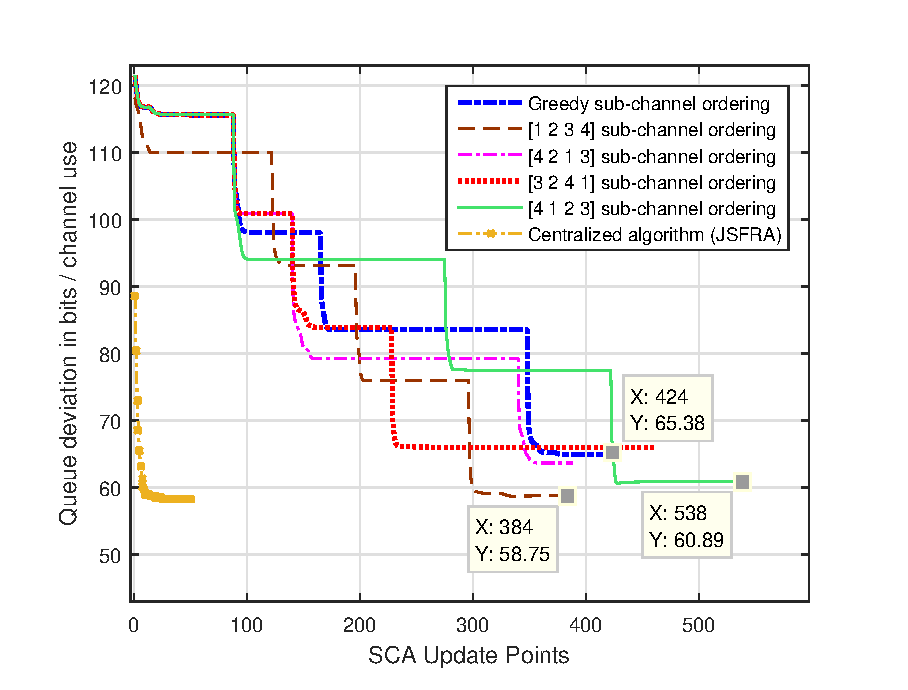
\includegraphics[width=0.8\textwidth]{reviewer_2_Q1A.eps}
		\label{fig-review-1b}
	}
	\caption{Convergence of the algorithms for \me{\lbrace N,N_B,K,N_T,N_R \rbrace = \lbrace 4,2,12,4,1 \rbrace} using \me{\ell_1} norm}
	\label{fig-review-1}
\end{figure*}

We remark that the choice of a sub-channel ordering scheme should also consider the number of backlogged packets associated with each user. We have emphasized this issue by comparing various ordering schemes for the same system model with two different set of backlogged packets associated with each user. We do not include the following figures in the manuscript due to space limitations, nevertheless, we have included in the response letter to answer the reviewers' question. We considered a system with \eqn{N = 4} sub-channels, \eqn{N_B = 2} \acp{BS} with \eqn{N_T = 4} transmit antennas and \eqn{K = 12} single antenna users. The \ac{PL} is distributed uniformly over \eqn{[0,-3]} dB. The number of backlogged packets assumed for each user is provided in the corresponding captions in Figure \ref{fig-review-1}.

Figure \ref{fig-review-1} compares different sub-channel ordering schemes in terms of the total number of backlogged packets remaining in the system. As can be seen from Figure \ref{fig-review-1}\subref{fig-review-1a}, the greedy sub-channel ordering provides a favorable way of choosing sub-channels to minimize the total number of backlogged packets. However for another scenario in Figure \ref{fig-review-1}\subref{fig-review-1b}, it is evident that the greedy sub-channel ordering is no longer better in comparison to the few other random ordering schemes. Note that the difference between the two scenarios is only the queue distribution, which are listed out in the corresponding figure caption. We have included the discussions regarding the greedy sub-channel ordering in the revised manuscript as a heuristic approach under Section III-D final paragraph. However, it is worth noting that as the number of users in the system increases, all sub-channel ordering schemes are similar in minimizing the total number of backlogged packets in the system without any noticeable gain.

\pagebreak
\cmnt{2} \review{The authors mentioned that the signaling overhead of the distributed algorithm can be reduced by using a smaller number of iterations \eqn{J_{\max}}. But still, you didn't answer my question about whether the signaling overhead of the distributed algorithm is smaller than the centralized algorithm. You should first analyze the signaling overhead of the distributed algorithm for fixed \eqn{J_{\max}} and the signaling overhead of the centralized algorithm. Then you should point out under what \eqn{J_{\max}} the distributed algorithm will have less signaling overhead than the centralized algorithm. Is it possible that the distributed algorithm always has more signaling overhead than the centralized algorithm even when \eqn{J_{\max} = 1}? Finally, there is a trade-off between performance and signaling overhead (\eqn{J_{\max}}) for the distributed algorithm. For the same signaling overhead (we can control \eqn{J_{\max}} to make the signaling overhead of the distributed algorithm approximately equal to that of the centralized algorithm), does the distributed algorithm achieve better performance than the centralized algorithm?}
	
\resp We apologize for the lack of clarity in explaining this information in our earlier submission. To answer this question in detail, we consider the following scenarios based on the channel correlation between the adjacent transmission instants. 

\begin{itemize}
\item At first we consider a semi-static scenario, where the channel remains constant for multiple transmission instants. Therefore, the \ac{CSI} information available at the transmitter or the centralized controller are valid for multiple transmission instants. In order to discuss the performance of the centralized and the distributed schemes, let us consider a system model with \eqn{N=4} sub-channels, \eqn{N_B = 3} \acp{BS}, each equipped with \eqn{N_T = 8} transmit antennas. Let \eqn{K = 12} be the number of users in the system equipped with \eqn{N_R = 1} receive antenna. Let the \ac{PL} between the \acp{BS} and the users are drawn uniformly between \eqn{[0,-3]} dB. Figure \ref{fig-review-2-a} plots the number of backlogged packets present in the system after each \ac{SCA} update point. Note that for \eqn{J_{\max} > 1}, each \ac{SCA} points includes \eqn{J_{\max}} number of \ac{ADMM} iterations performed. Therefore, it needs to be considered while analyzing the signaling overhead. Note that we consider only \ac{ADMM} based distributed approach outlined in Algorithm 2.
\begin{figure}[h!]
\centering
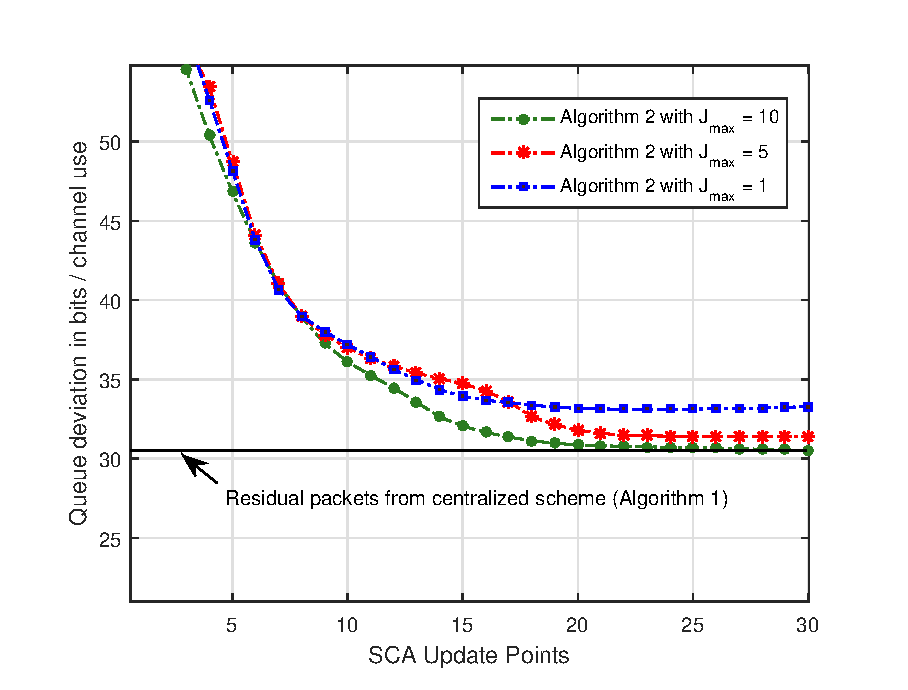
\includegraphics[width=0.8\columnwidth]{reviewer_2_Q1C-B.eps}
\caption{Convergence of the centralized and distributed algorithms for \me{\lbrace N,N_B,K,N_T,N_R \rbrace = \lbrace 4,3,12,8,1 \rbrace} using \me{\ell_1} norm with the backlogged packets as \eqn{Q_k = [17,7,14,14,12,14,8,13,8,11,9,12]} bits}
\label{fig-review-2-a}
\end{figure}

Let us consider the centralized configuration, in which the \ac{CSI} required to be exchanged between \acp{BS} and the centralized controller. In order to quantify the amount of signaling overhead, let us consider that each real entity of the complex channel is represented by \eqn{N_C = 10} bits.\footnote{Note that \eqn{N_C = 10} bits can be justified for the \ac{CSI} quantization, since the precoders are designed based on the quantized \ac{CSI} fed back from the \acp{BS} to the centralized controller.} Using this information, the amount of signaling required to be exchanged between \acp{BS} and the centralized controller is given by \eqn{N \times N_B \times N_T \times K \times 2} real entities, which is equal to \eqn{23,040} bits. In addition, we also need the precoder signaling from the centralized controller to all \acp{BS}. It accounts to \eqn{N \times K \times N_T \times 2} real entities, which is equal to \eqn{7,680} bits. On the whole, it requires \eqn{30,720} bits that needs to be exchanged via backhaul over \eqn{T} transmission slots, where \eqn{T} denotes the number of slots for which the channel remains constant. Additionally, we also need to update the queue information to the controller in each transmission instant and the updated precoders are required to be transmitted back. Therefore, even though the \ac{CSI} is not required to be signaled to the controller, the precoders are fed back to all \acp{BS} in each transmission slot based on the current backlogged packets, which are updated by all \acp{BS} to the controller. Even though, we are not using quantized \ac{CSI} in our performance evaluation, it is worth noting that the achievable gains deteriorates significantly if the precoders are designed using the quantized \acp{CSI} [R1].

On contrary, the distributed approach based on \ac{ADMM} requires only the exchange of coupling interference variables that are scalar values. For a fully connected network, each consensus variable binds only two \acp{BS} only, therefore, the overall number of entities that needs to be exchanged is \eqn{N \times (N_B - 1) \times K \times 2} real entries, which is equal to \eqn{960} bits by considering \eqn{N_D = 5} bits to represent the scalar coupling variables. Note that \eqn{5} bits are more than sufficient for representing the interference variables since they are bounded by the transmit power. Therefore, in each transmission instant, the overall signaling required to design the precoders jointly requires \eqn{J_{\max} \times I_{\max} \times 960} bits. Note that there is no need to exchange the backlogged packets to the coordinating \acp{BS} in the distributed scheme. Note that \eqn{I_{\max}} denotes the number of \ac{SCA} iterations and \eqn{J_{\max}} represents the inner \ac{ADMM} update steps.

Now, let us consider the performance of \ac{ADMM} based distributed precoder design for different \eqn{J_{\max}} values as in Figure \ref{fig-review-2-a} for analyzing the signaling overhead required and the performance improvement from the exchange of information. The centralized scheme is given as a lower bound in Figure \ref{fig-review-2-a}, since the \acp{CSI} available at the controller can be used to design the precoder until convergence. Figure \ref{fig-review-2-a} shows noticeable improvement in the reduction of number of backlogged packets in the system as we increase the number of \ac{ADMM} iterations. However, note that as we increase the number of iterations, the signaling requirement also grows with the factor of \eqn{J_{\max}}. 

From Figure \ref{fig-review-2-a}, it is evident that the \ac{ADMM} with \eqn{J_{\max} = 1} requires \eqn{I_{\max} = 15} iterations to perform close enough to the centralized scheme. In order to reach the performance close enough to that of centralized scheme, using above assumptions, it requires \eqn{960 \times 15 = 14,400} bits to be exchanged among the coordinating \acp{BS}. Note that it is \eqn{\approx 0.62} times the overhead involved in the centralized scheme to feedback only the \acp{CSI} to the controller, assuming single transmission instant. However, since the channel remains constant for certain duration, say \eqn{T}, the centralized approach may be favorable for this type of scenario. It is worth noting that the precoder exchange, which is required at each instant due to the changing traffic, involves significant overhead that also needs to be accounted while considering the selection.

However, if the channel changes once in every three transmission instants, \textit{i.e.}, the fed back \ac{CSI} is valid only for \eqn{T = 3}, then the distributed methods with \eqn{J_{\max} = 1} is preferred to the centralized approaches. The duration of the \ac{CSI} validity is evaluated using \eqn{B_{CSI} + B_{P} \times T = B_D \times T}, where \eqn{B_{CSI} = 23,040} denotes the number of bits required for the \ac{CSI} feedback, \eqn{N_C \times B_P = 7,680} corresponds to the number of bits required for the precoder feedback from the controller, and \eqn{B_D = 14,400} refers to the number of bits required to exchange the coupling interference variables in the distributed scheme. 

In general, the choice of selecting the centralized scheme over the decentralized approach depends on the factor \eqn{\Gamma} defined as
\begin{equation}
\Gamma \triangleq \left (\frac{N_C}{N_D} \right ) \times \frac{N_T \, (N_B + T)}{T \, (N_B - 1)}
\end{equation}
where \eqn{T} represents the duration over which the \ac{CSI} is valid for designing the precoders by the centralized controller. Note that we considered different quantization scales for the centralized and the distributed exchanges. If the fraction is \eqn{\Gamma > 1}, then the distributed scheme is preferred and if \eqn{\Gamma < 1}, then the centralized overhead is smaller and therefore, it is preferred. Note that we considered the distributed algorithms are iterated for the same count in each transmission slot. It is worth noting that since the channel is semi-static, the distributed schemes are not required to iterate for the same number of iterations in each transmission instant. Since the operating point can be chosen to be the solution obtained from the previous transmission instant, the convergence speed of the distributed algorithm can be accelerated significantly by doing so. 

Note that the above discussions does not include the overhead involved in the queue transfers to the controller and the loss in performance due to the distributed approach. The loss involved in the centralized performance due to the quantized \ac{CSI} is also not considered. Therefore, by using the above arguments, if the system size grows, \textit{i.e.}, as the number of transmit antennas increase, then the distributed approach is preferred to the centralized scheme even if the channel remains constant for longer duration such that \eqn{\Gamma > 1}. The reason is that the overhead involved in feeding back the precoders from the centralized controller will be significantly large.

In practice, it is not required to perform the distributed approaches for higher number of iterations [Chapter 3.2.2, 10]. According to the results in Figure \ref{fig-review-2-a}, it is sufficient to iterate for \eqn{I_{\max} = 10, J_{\max} = 1} iterations to achieve acceptable performance improvement from the coordinated precoder design. The reason is that the performance gained by exchanging additional coupling variables is marginal compared to the overhead involved in doing so.

\item Secondly, we consider a time-correlated fading scenario, where the channel changes slowly over each transmission instant based on the user mobility or the surrounding environment. In such cases, the pilots are periodically sent from each user to measure the \ac{CSI} by each \acp{BS} to design the precoders efficiently. In such scenarios, where the channel cannot be assumed constant over multiple transmission instants, the distributed schemes are much preferred to the centralized approaches. One such analysis was studied in Section C of [12] using dual decomposition based distributed precoder design, where they have showed that it is enough to follow the fading process to obtain desired performance instead iterating until convergence. Using this argument, it is beneficial to just follow the fading process by using the precoders designed in the previous transmission as the operating point for the current instant for \ac{SCA} rather starting at some random feasible point. 

Studying the performance of distributed algorithms for the time correlated case is beyond the scope of our paper and thus is not considered in the current manuscript. However, we take this opportunity to show a plot demonstrating this behavior for the \ac{KKT} based algorithm presented in Section IV-C of the manuscript. Note that there is no need for the backhaul exchange to design the precoders in the \ac{KKT} scheme proposed in Algorithm 3. However, it requires the exchange of information via \ac{OTA} transmissions using precoded pilots as discussed in Section IV-C.
\begin{figure}[h!]
	\centering
	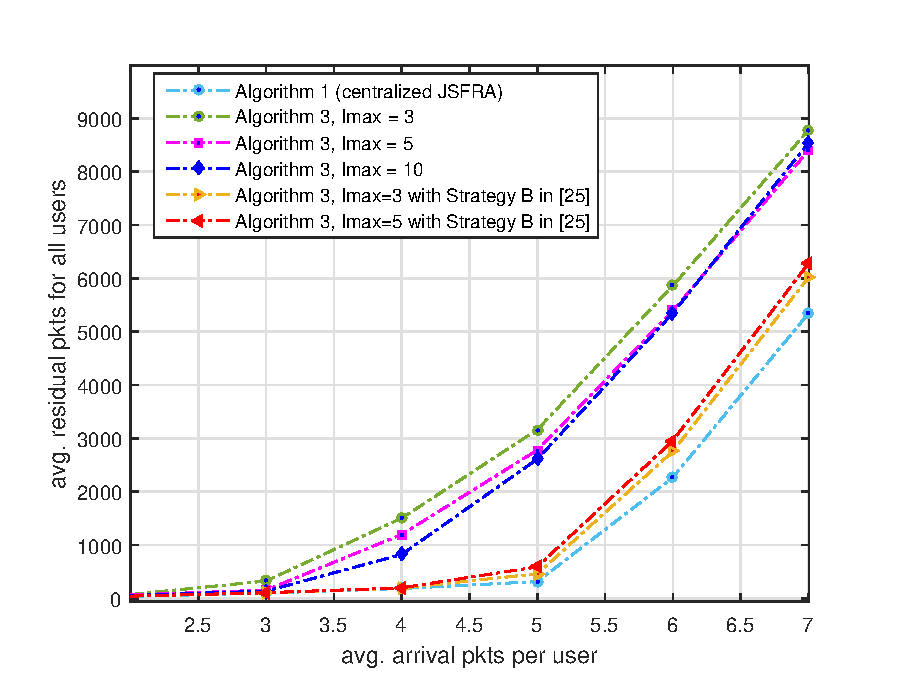
\includegraphics[width=0.8\columnwidth]{reviewer_2_Q2A.eps}
	\caption{Expected number backlogged packets after each transmission instant for a system \me{\lbrace N,N_B,K,N_T,N_R \rbrace = \lbrace 4,2,16,4,2 \rbrace} evaluated for \eqn{500} slots and \ac{PL} is distributed \eqn{\mathbb{U}(0,-3)}}
	\label{fig-review-2}
\end{figure}

Figure \ref{fig-review-2} compares the performance of the distributed \ac{KKT} approach, \textit{i.e.}, Algorithm 3 for different values of \eqn{I_{\max}}. The signaling requirements are outlined in Algorithm 3 and the overhead involved in the signaling is penalized in the achievable rate of the users.\footnote{Please refer to [25] for further details.} We considered that the channel is coherent over \eqn{N_S = 100} symbols and the precoder update is performed by exchanging the required information for \eqn{I_{\max} = 3,5,10}. The overhead is considered as \eqn{\tilde{t}_{l,k,n} = (1 - \frac{I_{\max}}{N_S}) \times t_{l,k,n}}, where \eqn{\tilde{t}_{l,k,n}} is the rate seen by the user and the factor \eqn{(1 - \frac{I_{\max}}{N_S})} is considered as a penalty involved due to the precoded pilot exchange. More details can be found in [R2] and [R3]. The average number of backlogged packets after each transmission slot is evaluated as 
\begin{equation}
\chi = \sum_{k = 1}^K \; [ Q_k - \tilde{t}_k ]^+
\end{equation}
and the \ac{PL} is distributed uniformly between \eqn{[0,-3]} dB.

Unlike Algorithm 3, the centralized precoder design presented in Figure \ref{fig-review-2} does not include any penalty term and it is used as a benchmark. In order to improve the performance of the distributed scheme, the operating point involved in the \ac{SCA} algorithm is considered from the earlier frame instead of being generated randomly. Note that the performance of the distributed scheme is significantly improved by performing the internal iterations as discussed in [25] as strategy B. By doing so, we can achieve the performance close enough to the centralized approach (which does not included any penalty term in the rate). Therefore, for the time-correlated scenarios, it would be beneficial to do distributed approaches as discussed above to avail the channel correlation rather than feeding back the \acp{CSI} to the centralized controller.

\end{itemize}	

\vspace{1eM}
[R1] Muhammad-Fainan Hanif, Le-Nam Tran, Antti T\"{o}lli, Markku Juntti,  and Savo Glisic, "{Efficient Solutions for Weighted Sum Rate Maximization in Multicellular Networks With Channel Uncertainties}'', \textit{IEEE Trans. Signal Process}., vol 61, no. 22, pp. 5659-5674, Nov. 2013.

[R2] Changxin Shi, Berry R.A., Honig M.L., ``{Bi-Directional Training for Adaptive Beamforming and Power Control in Interference Networks}," \textit{IEEE Transactions on Signal Processing}, vol.62, no.3, pp.607,618, Feb.1, 2014

[R3] P. Jayasinghe, A. T\"{o}lli, J. Kaleva,  M. Latva-aho, "{Bi-directional Signaling for Dynamic TDD with Decentralized Beamforming}'', in \textit{Proceedings of IEEE ICC SmallNets Workshop}, London, UK, June, 2015		

\vspace{1eM}		

The discussions are described in a condensed form in the first paragraph of Section IV and in the first and the last paragraph of Section IV-C. 

\begin{comment}


	\resp
	We thank the reviewer for the insightful comment and we apologize for the lack of clarity in explaining this information in our earlier manuscript. The answer to this question, we need to consider the following scenarios.
	\begin{enumerate}
	\item[(i)] How big is the system configuration and
	\item[(ii)] How fast the channel varies in relation to the transmit frame duration, \textit{i.e.}, whether the channel is semi-static (where the \ac{CSI} remains almost constant for multiple transmission slots) or time-correlated (where the channel changes over each transmission slot with some memory).
	\end{enumerate}
	
	\begin{itemize}
		
	\item Based on the condition (i), we can discuss the possibilities of the centralized schemes over the distributed methods using the amount of signaling overhead involved in the precoder design.
	
	\begin{enumerate}
	\item The amount of signaling required for the distributed algorithms and the centralized ones depend on the system configuration under consideration. For example, let us consider a model with \eqn{N = 1} sub-channel, \eqn{K = 4} users and \eqn{N_B = 2} \acp{BS}, each serving 2 users. Let \eqn{N_T = 4} be the number of transmit antennas and \eqn{N_R = 1} be the number of receive antennas at each user. We note that a centralized algorithm requires the knowledge of all channels matrices in the system and thus the resulting amount of information exchange is proportional to the product of the numbers of users (\eqn{K}), \acp{BS} (\eqn{N_B}), and transmit and receive antennas (\textit{i.e.}, \eqn{N_T} and \eqn{N_R}).
	
	In order to quantify the total number of bits required for a centralized solution, let us assume that each scalar complex channel component requires \eqn{10} bits, \textit{i.e}, \eqn{4} bits for amplitude and \eqn{6} bits for phase (assuming phase is more important) or it can be a equal share of \eqn{5} bits for both amplitude and phase. Using this assumption, the total number of bits for channel information to be exchanged via backhaul is \eqn{10 \times K \times N_B \times N_R \times N_T = 320} bits. On the other hand, for the distributed algorithms, let us consider \eqn{6} bits for quantizing each element of the real-valued coupling variables. Consequently, the proposed distributed solutions require \eqn{6 \times 2 \times 2} bits to be exchanged in each iteration. Note that here we consider the distributed approaches discussed in Sections IV-A and IV-B only, since the \ac{KKT} based approach involves the precoded pilot transmissions to update the corresponding precoders and receivers.
	
	In the above scenario, for the same amount of signaling overhead as that of the centralized schemes, we can perform only 6 \ac{SCA} updates with \eqn{J_{\max} = 2} (\textit{i.e.}, two updates for \ac{ADMM} part). This may not be sufficient for the distributed algorithms to attain the same performance as that of the centralized methods. However, as the number of sub-channels, users and/or the antenna elements increases, it may not be a feasible option to send complete \acp{CSI} across the coordinating \acp{BS} to the centralized controller in the current cellular systems. 
	
	In addition to comparing the signaling overhead, we also need to consider the performance loss due to the \ac{CSI} quantization in the centralized approaches, which is beyond the scope of our paper. Generally, the performance is significantly degraded if precoders are designed with the quantized \ac{CSI} as discussed in [R1]. Moreover, in the centralized algorithm, resulting transmit precoders need to be exchanged with the corresponding \acp{BS} before the actual transmission, which involves significant overhead in the backhaul usage. Using the above discussion, we can say that for a small sized systems, centralized algorithm would be preferable as compared with the distributed schemes.
	
	\vspace{1eM}
	[R1] Muhammad-Fainan Hanif, Le-Nam Tran, Antti T\"{o}lli, Markku Juntti,  and Savo Glisic, "{Efficient Solutions for Weighted Sum Rate Maximization in Multicellular Networks With Channel Uncertainties}'', \textit{IEEE Trans. Signal Process}., vol 61, no. 22, pp. 5659-5674, Nov. 2013.
	\vspace{1eM}		

	\item However, for a system involving more coordinating \acp{BS}, users and antenna elements, it would be preferable to use the distributed algorithms for designing the precoders independently across the coordinating \acp{BS}. It can be justified by using Figure. \ref{fig-review-2-a}, which compares the total number of backlogged packets present in the system after each \ac{SCA} update. Note that for the sake of clarity, we have plotted only the number of backlogged packets at each \ac{SCA} points. 
	
	Let us consider the system in Figure \ref{fig-review-2-a} for the overhead analysis. It requires \eqn{N=4 \times N_B=2 \times K=12 \times N_T=4 \times N_R=1 = 384} complex channel components to be exchanged between \acp{BS} to the controller for the centralized approach to design the precoders. Additionally, it also requires to transmit the precoders back to the \acp{BS} upon convergence of the algorithm, which requires \eqn{N = 4 \times K=12\times N_T = 4 \times = 192} complex precoder components. Now, assuming \eqn{10} bits are used to quantize each real entity, it requires \eqn{11520} bits to be exchanged overall to obtain the performance shown in Figure \ref{fig-review-2-a}.
	\begin{figure}[h!]
		\centering
		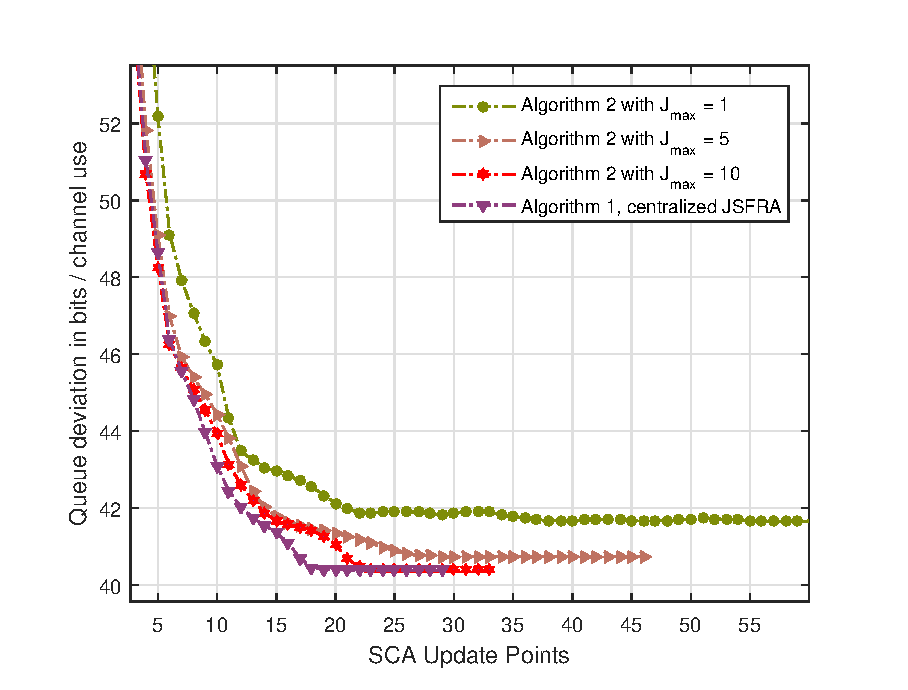
\includegraphics[width=0.8\columnwidth]{reviewer_2_Q1C-A.eps}
		\caption{Convergence of the centralized and distributed algorithms for \me{\lbrace N,N_B,K,N_T,N_R \rbrace = \lbrace 4,2,12,4,1 \rbrace} using \me{\ell_1} norm with the backlogged packets as \eqn{Q_k = [10,9,6,11,7,9,9,10,7,8,6]} bits}
		\label{fig-review-2-a}
	\end{figure}
	On contrary, for the distributed \ac{ADMM} case, real valued coupling interference variables are required to be exchanged among the coordinating \acp{BS} in the network. For the system scenario used in Figure \ref{fig-review-2-a}, the scalar interference values that needs to be exchanged across the coupling \acp{BS} is \eqn{N=4 \times K = 12 \times N_B = 2 = 96} real values. Assuming \eqn{10} bits are required to quantize the scalar interference values, on the whole, in each exchange it requires \eqn{960} bits among the coordinating \acp{BS}. However, note that in practice we do not need \eqn{10} bits to quantize the scalar interference values, since they are bounded by the total transmit power, unlike the channel coefficients that has a large dynamic range due to \ac{PL}.
	
	Now, assuming \eqn{J_{\max} = 1}, we require \eqn{1920} bits, \textit{i.e.}, roughly \eqn{\ith{\tfrac{1}{6}}} of the overhead involved in the centralized approach to reach the backlogged packets of \eqn{42} bits. Note that the loss in the performance is only \eqn{2} bits over the centralized approach, whereas the gain in reducing the overhead is \eqn{9600} bits over the centralized scheme. Similarly, for \eqn{J_{\max} = 5} case, it requires \eqn{15} iterations to achieve \eqn{42} bits of backlogged packets, and therefore the overhead is roughly around \eqn{7200} bits (it includes 5 inner \ac{ADMM} iterations as well) which is roughly \eqn{1.6} times less than the centralized scheme. Therefore, as the system size increases, the performance improved from the centralized scheme by exchanging \ac{CSI} information becomes marginal compared to the reduction in the backlogged packets.

	However, it is worth noting that \ac{ADMM} with \eqn{J_{\max} = 1} is not monotonic, and therefore it is difficult to prove the convergence theoretically, despite being the preferable approach for practical implementation.
	\end{enumerate}

	\item Now, based on condition (ii), the selection between the centralized and the distributed approaches are argued as follows. 
	
	\begin{enumerate}
	
	\item If the channel is semi-static, \textit{i.e.}, the \acp{CSI} exchanged by the coordinating \acp{BS} to the centralized controller are valid for multiple transmission frames, then it would be beneficial to choose centralized schemes. It follows from the fact that the controller can update the beamformers based on the instantaneous backlogged packets, and the \acp{CSI} are available from the earlier feedback. Note that the \acp{CSI} are still valid due to the static nature of the channel seen between any two entities in the network.
	
	\item However, in reality, since the channel is time-correlated, it is enough to update the precoders once per radio frame. Thus, it is not necessary for the distributed algorithm to converge until the end. Instead, the decentralized parts only need to follow the fading process when \eqn{J_{\max} > 1}. The performance of the distributed algorithm based on the dual decomposition scheme was discussed for the time-correlated fading in Section C of [12], which showed that it is enough for the distributed precoder design to follow the fading process to provide the desired performance. Studying the performance of distributed algorithms for the time correlated case is beyond the scope of our paper and thus is not considered in the current manuscript. However, we take this opportunity to show a plot demonstrating this behavior for the \ac{KKT} based algorithm presented in Section IV-C of the manuscript.
	\begin{figure}[h!]
		\centering
		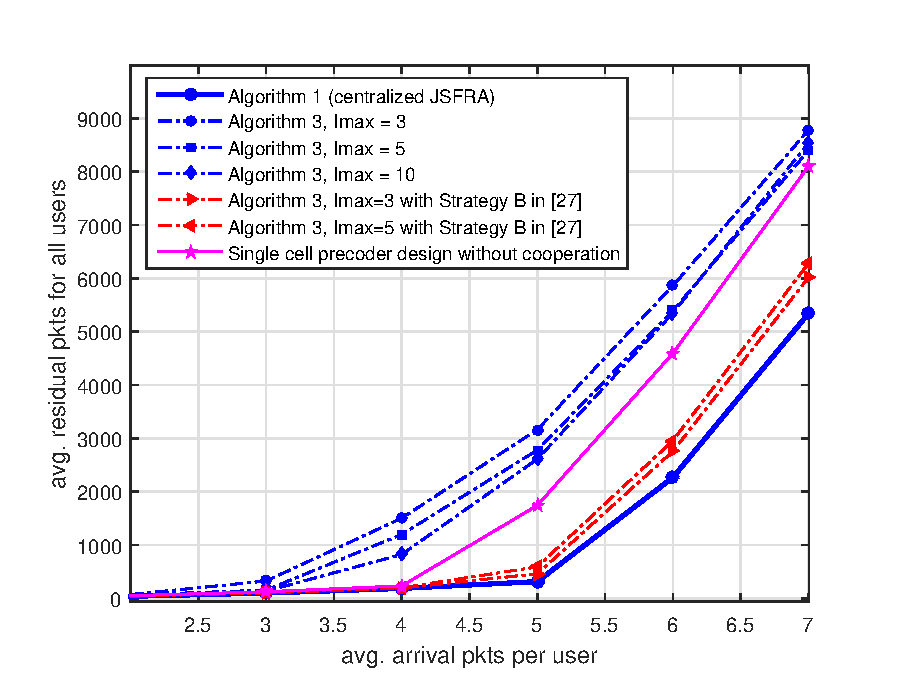
\includegraphics[width=0.8\columnwidth]{reviewer_2_Q2.eps}
		\caption{Expected number backlogged packets after each transmission instant for a system \me{\lbrace N,N_B,K,N_T,N_R \rbrace = \lbrace 4,2,16,4,2 \rbrace} evaluated for \eqn{500} slots}
		\label{fig-review-2}
	\end{figure}
	
	Figure \ref{fig-review-2} compares the performance of the distributed \ac{KKT} approach, \textit{i.e.}, Algorithm 3 for different values of \eqn{I_{\max}}. The signaling requirements are outlined in Algorithm 3 and the overhead involved in the signaling is penalized in the achievable rate of the users.\footnote{Please refer to [27] for further details.} We considered that the channel is coherent over \eqn{N_S = 100} symbols and the precoder update is performed by exchanging the required information for \eqn{I_{\max} = 3,5,10}. The overhead is considered as \eqn{\tilde{t}_{l,k,n} = (1 - \frac{I_{\max}}{N_S}) \times t_{l,k,n}}, where \eqn{\tilde{t}_{l,k,n}} is the rate seen by the user and the factor \eqn{(1 - \frac{I_{\max}}{N_S})} is considered as a penalty involved due to the precoded pilot exchange. More details can be found in [R2] and [R3]. The average number of backlogged packets after each transmission slot is evaluated as 
	\begin{equation}
	\chi = \sum_{k = 1}^K \; [ Q_k - \tilde{t}_k ]^+
	\end{equation}
	and the \ac{PL} is distributed uniformly between \eqn{[0,-3]} dB.
	
	Unlike Algorithm 3, the centralized and the isolated precoder designs presented in Figure \ref{fig-review-2} does not include any penalty term and it is used as a benchmark. In order to improve the performance of the distributed scheme, the operating point involved in the \ac{SCA} algorithm is considered from the earlier frame instead of being generated randomly. Note that the performance of the distributed scheme is significantly improved by performing the internal iterations as discussed in [25] as strategy B. By doing so, we can achieve the performance close enough to the centralized approach (which does not included any penalty term in the rate). Therefore, for the time-correlated scenarios, it would be beneficial to do distributed approaches as discussed above to avail the channel correlation rather than feeding back the \acp{CSI} to the centralized controller.
	
	Since we use \ac{KKT} approach, we can either use all users in the system for the precoder design or we can utilize single-cell MU-MIMO user selection presented in the literature to limit the number of users for which the precoders are designed, which leads to the faster convergence. As we can see from Figure \ref{fig-review-2}, as the arrival rate per user increases, the performance of \ac{KKT} schemes with \eqn{J_{\max} = 3,5,10} converges since the number of backlogged packets are significantly large, therefore, the same set of users will be served by the algorithm with better precoders by utilizing the memory. 
	
	In spite of using memory and prior scheduling in the \ac{KKT} approach, isolated single \ac{BS} processing performs much better than the distributed scheme due to the limited number of iterations allowed in the algorithm. Note that the precoders are not updated for the desired users until convergence, after the limited number of iterations. However, if we perform the single cell precoder design by considering the neighboring precoders as fixed after the recent exchange as discussed in [28], we can improve the performance significantly for Algorithm 3 as shown by red curves in Figure \ref{fig-review-2}. In this approach, in between each exchange across the coordinating \acp{BS}, each \ac{BS} will perform \eqn{J_{\max} = 20} with the neighboring precoders as fixed. Once the iterations are performed to update the precoders, it is then exchanged across the coordinating \acp{BS} to perform the same procedure as mentioned earlier. 
	
	\vspace{1eM}
	[R2] Changxin Shi, Berry R.A., Honig M.L., ``{Bi-Directional Training for Adaptive Beamforming and Power Control in Interference Networks}," \textit{IEEE Transactions on Signal Processing}, vol.62, no.3, pp.607,618, Feb.1, 2014
	
	[R3] P. Jayasinghe, A. T\"{o}lli, J. Kaleva,  M. Latva-aho, "{Bi-directional Signaling for Dynamic TDD with Decentralized Beamforming}'', in \textit{Proceedings of IEEE ICC SmallNets Workshop}, London, UK, June, 2015		
	\vspace{1eM}
		
	\end{enumerate}
			
	\end{itemize}
			
\end{comment}			
				
\pagebreak
\cmnt{3} \review{If the authors can't prove the convergence of the ADMM algorithm (or the decomposition approach via KKT conditions) in Section IV.B, then at least, you should discuss the property of the fixed point of the algorithm. For example, does there exist a fixed point of the algorithm? If so, is the fixed point of the algorithm unique? Is any fixed point of the algorithm also the optimal solution of the original problem in (20)? Assuming that the ADMM algorithm converges to a fixed point, will the interference vector in (39) converges to the actual interference in the network? These questions must be clarified in the paper. Otherwise, it is not clear how the ADMM algorithm is related to the original problem in (20). Similar questions should also be answered for the decomposition approach via KKT conditions. }

\resp We thank the reviewer for raising the concern regarding the convergence of the distributed algorithms. We have substantially improved the clarity of both primal and the \ac{ADMM} based approach in the revised manuscript (see Appendix B). There, we have utilized the strong convexity of the objective function to ensure the uniqueness of the minimizer in each \ac{SCA} step. Additionally, since each subproblem in (20) or (28) has a convex feasible set, the convergence of the \ac{ADMM} scheme is guaranteed by using [10] and [36, Prop. 4.2] as discussed in Appendix B. 

In our paper, the number of \ac{ADMM} iterations is denoted by \eqn{J_{\max}} in Algorithm 2. In order to obtain the centralized solution, we need to perform the distributed approaches until convergence or for some finite number, say, \eqn{J_{\max}}. In practice, it may not be possible to perform the distributed methods until convergence. In such cases, the overall convergence of the objective sequence and beamformer iterates of Algorithm 2 cannot be guaranteed. It follows from the fact that in each distributed step, the global objective need not decrease strictly to ensure the convergence of the beamformer iterates.

However, if we perform the distributed algorithms for significant number of iterations to ensure strict monotonicity of the objective, then the overall of convergence of Algorithm 2 is guaranteed by following the arguments in [27]. Note that in addition, uniqueness of the limit point is also necessary for the sequence convergence. It is achieved by regularizing the original convex objective with a quadratic term as in (46b) in each \ac{SCA} step to guarantee strong convexity, and thereby ensuring unique minimizer and limit point. 

Upon satisfying the strict monotonicity of the objective sequence in each \ac{SCA} update with some \eqn{J_{\max}}, we can also combine the \ac{MMSE} receiver update in (23b) after each \ac{SCA} step for the transmit precoders. It reduces the signaling overhead involved with the information exchange due to multiple loops that are required for \ac{AO} and \ac{SCA} as mentioned for the centralized scheme. Even though the receivers are updated together with the transmit precoders in each \ac{SCA} step, strict monotonicity of the objective sequence is still ensured. It follows from the fact that the \ac{MMSE} receivers are optimal for fixed transmit precoders obtained after each \ac{SCA} update. Moreover, the newly found solution is also feasible and the objective improves monotonically in strict sense. Therefore, if the above conditions are satisfied, then the convergence of the sequence of iterates is guaranteed. 

For our simulation scenario, we have fixed the maximum number of \ac{ADMM} iterations in each \ac{SCA} step as \eqn{J_{\max} = 20}. Note that it is sufficient to ensure strict monotonic decrease of the objective value in each \ac{SCA} step. However, the number of iterations to ensure strict monotonicity of the objective depends on the problem under consideration. The practical significance of limited number of \ac{ADMM} iterations is discussed briefly in [10, Section 3.2.2].

Regarding the specific comments related to the \ac{ADMM} convergence for subproblem (20), we provide the following remarks by considering that the objective is regularized by a quadratic term as discussed in Appendix A-B to ensure strongly convexity.

\begin{enumerate}
\item The primal objective and the augmented Lagrangian are strongly convex, therefore, the optimal solution exists and is unique in the feasible convex set of subproblem (20). It follows from that the \ac{ADMM} algorithm converges to a unique limit point, which is a fixed point of the iterative \ac{ADMM} algorithm.

\item In general, the fixed point of the subproblem (20) is not unique. It is due to the fact that the original objective is not strongly convex, thereby having possibly multiple solutions in the feasible convex set. It is due to the existence of multiple solutions, the \ac{ADMM} algorithm can have a set of fixed points in the feasible set. However, if we regularize the objective with a strongly convex quadratic term as discussed in Appendix A-B, then the distributed approaches find a unique fixed point of the original convex subproblem.

\item By using previous argument, any fixed point of the algorithm is a solution for the problem (20), since all fixed points are in fact the solution for the convex subproblem in (20). The particular choice of the fixed point of the \ac{ADMM} approach depends on the initial operating point used in the regularization term in the objective.

\item Upon convergence of the \ac{ADMM} approach, the interference vector is guaranteed to be equal to the actual interference seen in the network. This is the main principle of \ac{ADMM} where the local variables (the vectors in (38)) converge to the global variables, which are the actual inference vectors.

\end{enumerate}

However, if the reviewer comments are for the Algorithm 2, then the following response will answer the questions. For that, we consider the following conditions are satisfied in each \ac{SCA} update step.
\begin{itemize}
	\item The objective function is regularized by a quadratic term as discussed in Appendix A-B to ensure strict convexity of the objective function, which leads to the uniqueness of the solution.
	\item The distributed algorithms are performed until convergence or for sufficient number of iterations to ensure strict monotonic decrease of the objective sequence.
\end{itemize}
Upon satisfying the above conditions, even if we update the receive beamformers using the \ac{MMSE} receiver in (23b) after each \ac{SCA} step for solving the transmit precoders, strict monotonicity is still ensured. It follows from the fact that the \ac{MMSE} receivers are optimal for the fixed transmit precoders, and therefore the objective sequence decreases monotonically after each update in strict sense.

\begin{enumerate}
	\item Since the above conditions are satisfied by Algorithm 2, then the existence of a fixed point for Algorithm 2 is guaranteed by following the arguments in [27].
	
	\item In general, fixed point of Algorithm 2 is not unique. Note that the iterative nature of the \ac{SCA} approach is based on approximating the nonconvex constraint by a convex one around some fixed operating point. While initializing the iterative Algorithm 2, we need to find a fixed operating point upon which the convex function is approximated. Therefore, depending on the choice of initial feasible point, the algorithm terminates at different fixed point upon convergence. Hence, there exist a set of fixed points for Algorithm 2.
	
	\item The nonconvex problem (16) can have multiple stationary points and the iterative method proposed in Algorithm 2 finds a stationary point of the nonconvex problem. Therefore, all fixed points found by Algorithm 2 upon convergence are indeed the stationary points of the original nonconvex problem.
		
	\item Upon convergence of the \ac{ADMM} approach, the interference vector is guaranteed to be equal to the actual interference seen in the network. This is the main principle of \ac{ADMM} where the local variables (the vectors in (38)) converge to the global variables, which are the actual inference vectors.
	
\end{enumerate}

On the other hand, the iterative method described in Algorithm 3 is based on a heuristic iterative approach to find a solution of \ac{KKT} equations, we cannot prove its convergence. When Algorithm 3 terminates, we will use the transmit and receive beamforming vectors to calculate the original objective. Based on the reviewer comments, we have mentioned that the convergence of the Algorithm 3 cannot be proved theoretically (see Appendix B last paragraph).

We have updated the manuscript to clarify all the points mentioned above. Please refer to Section IV-B last paragraph after (40) in the revised manuscript. Additional information regarding the convergence of the distributed algorithms is provided in Appendix B second paragraph. The discussion on the convergence of the KKT based approach for MSE reformulation scheme is also presented in Appendix B last paragraph. For reference purpose, we have also referred the interested reader to [10], which discusses exclusively about the \ac{ADMM} approach.

\begin{comment}
\resp We thank the reviewer for raising the concern regarding the convergence of the distributed algorithms with limited number of iterations. In view of this, we have updated the manuscript to include discussions on the convergence of the distributed algorithms with a limited number of iterations in the third paragraph of Appendix B after (57). Since the monotonicity of the algorithm with limited number of updates in each subproblem is not guaranteed in each iteration, it is hard to prove the convergence of the overall algorithm. However, if the algorithm is allowed to converge or iterated enough to guarantee the strict monotonicity of the objective in between the \ac{SCA} updates, the global convergence of the algorithm to a limit point of the original nonconvex problem is guaranteed based on the discussions provided in Appendix A.
\begin{itemize}
\item If there exists a fixed point or a set of fixed points for the original nonconvex problem in (16), then the proposed centralized algorithm in Section III-B and III-C finds at least one such point if iterated until convergence, which is provided in Appendix A. In order to find a unique fixed point, we regularize the objective function in (16) with a quadratic penalty term as discussed in Appendix A to transform the objective as a strongly convex function.
\item If the distributed algorithm is carried out for a limited number of iterations, it is not guaranteed to achieve a fixed point even if the outer \ac{SCA} update is performed for a large number of iterations. By this approach, the distributed approaches are not guaranteed to converge to a stationary point. In all our simulations on the primal and the \ac{ADMM} approach, we have set \eqn{J_{\max} = 20} in order to guarantee the monotonicity of the objective.
\item Unless the objective function is regularized with a strongly convex term as in Appendix A-C, the uniqueness of the iterates is not guaranteed. 
\item In each \ac{SCA} update, if the distributed algorithms are allowed to converge to the centralized solution, then the overall convergence will be a stationary point of the original nonconvex problem by following the same argument as that of the centralized algorithm.
\item Since the coupling between the distributed precoder designs is the interference between the BSs and the users, in the \ac{ADMM} approach, the interference is treated as a local variable, which is then included in the precoder design problem for each coordinating BS. This is treated as a local variable for individual \acp{BS}. Note that the local variable is an assumption made by the BS on the actual interference caused by the neighboring BSs. Since the actual interference caused is different, the consensus has to be made between the local interference variable maintained at each BS with the global consensus interference variable, which is nothing but the average between the corresponding BSs interference. These discussions have been made in the revised manuscript in Section IV-B. For reference purpose, we have also referred the interested reader to [11], which discusses exclusively about the ADMM approach. Upon convergence of the \ac{ADMM} approach, the interference vector is equal to the actual interference seen in the network.
\end{itemize}

\end{comment}

\end{enumerate}
